% \UPSTIobjectif{

% }
\section{Présentation du système}
\subsection{Présentation générale}
L'étude de ce devoir porte sur la mise en place d'une programmation orientée objet sur un système simplifié de tri de pièces.
Le système est représenté sur la Figure \ref{fig:tri_de_piece} Ce système reçoit des pièces en provenance d'une chaine de production et les trie en fonction de leur taille. Plus précisément, les pièces arrivent depuis une goulotte inclinée jusqu'à un poste de mesure. Lorsque le convoyeur est libre, la pièce est transférée sur le convoyeur à l'aide du vérin \emph{VTRANS} puis est poussée dans un des bacs selon sa taille : \emph{PETIT}, \emph{MOYEN} ou \emph{GRAND}. Les pièces présentant un défaut restent sur le convoyeur jusqu'au bac 4 servant de mise au rebut.

\begin{figure}[h!t]
    \centering
    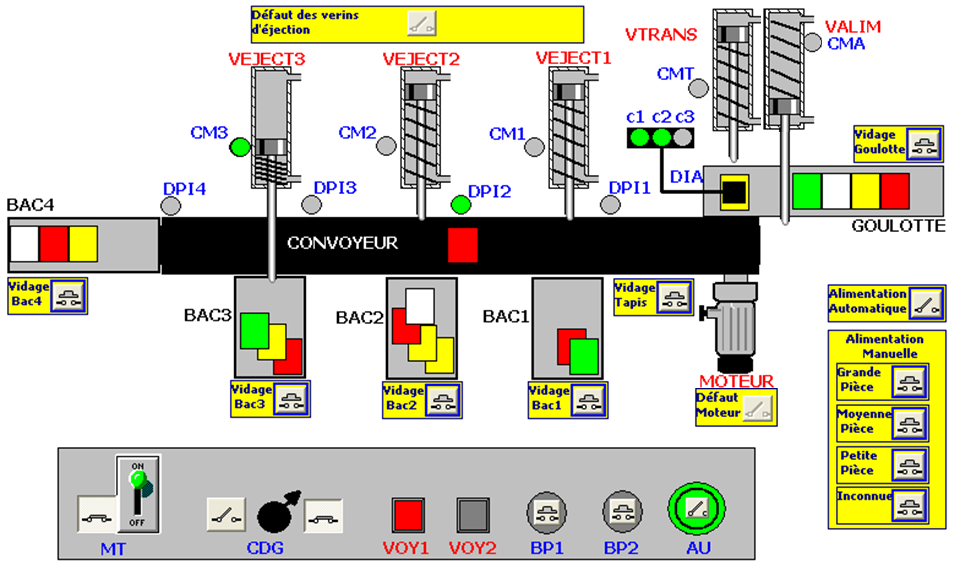
\includegraphics[width=0.8\linewidth]{tri_de_piece}
    \caption{Système de tri de pièces}
    \label{fig:tri_de_piece}
\end{figure}

\pagebreak
\section{Le poste de mesure -- transfert}
\subsection{Présentation}
L'étude se concentre sur la partie de la machine qui permet de mesurer la taille des pièces et de les transférer sur le convoyeur.

\begin{figure}
    \centering
    \adjincludegraphics[width=0.5\linewidth, clip, trim={0.64\width} {0.56\height} 0 0 ]{tri_de_piece}
    \caption{Poste de mesure et de transfert}
    \label{fig:poste_mesure}
\end{figure}

La liste des capteurs et actionneurs est donnée dans le tableau suivant :
\begin{center}
    \begin{tabular}{|l|p{0.33\textwidth}|p{.33\textwidth}|l|}
        \hline
        \multicolumn{4}{|c|}{\textbf{Capteurs}}\\ \hline
        \textbf{Nom} & \textbf{Type} & \textbf{Description} & \textbf{Variable}\\
        \hline
        \emph{CMA} & Logique & Capteur fin de course vérin Alim & ixAlimRentre \\ \hline
        \emph{CMT} & Logique & Capteur fin de course du vérin de Transfert & ixTransfertSorti \\\hline
         \emph{DIA} & Numérique & Capteur de hauteur de la pièce (cf Mesure des pièces ci-dessous) & \\ \hline\hline
         \multicolumn{4}{|c|}{\textbf{Actionneurs}}\\\hline
         \textbf{Nom} & \textbf{Préactionneur} & \textbf{Description}  & \textbf{Variable} \\
        \hline
         \emph{VALIM} & Vérin pneumatique simple effet, normalement sorti. Distributeur monostable. & Vérin de blocage des pièces sur la goulotte. & qxAlimRentrer \\ \hline
         \emph{VTRANS} & Vérin pneumatique simple effet normalement rentré. Distributeur bistable. & Vérin de transfert des pièces sur le convoyeur. & qxTransfertSortir \\\hline
    \end{tabular}
\end{center}

La mesure des pièces est faite par le capteurs \emph{DIA}. Il délivre trois signaux logiques \emph{C1}, \emph{C2} et \emph{C3} en fonction de la hauteur de la pièce. La table de correspondance est donnée dans le tableau suivant :

\begin{center}
    \begin{tabular}{|c|c|c|c|}
        \hline
        \textbf{Hauteur} & \textbf{ixC1} & \textbf{ixC2} & \textbf{ixC3} \\ \hline
        Petit & 1 & 0 & 0 \\ \hline
        Moyen & 1 & 1 & 0 \\ \hline
        Grand & 1 & 1 & 1 \\ \hline
    \end{tabular}
\end{center}
Toute autre combinaison de signaux devra considérer la pièce associée comme étant défectueuse. 

%%%% /Explication %%%%
